\documentclass{article}

\usepackage[utf8]{inputenc}
\usepackage[margin=1in]{geometry}
\usepackage[colorlinks=true, pdfborder={0 0 0}]{hyperref} 
\usepackage{microtype}
\usepackage{amsfonts}
\usepackage{amssymb}
\usepackage{graphicx}
\usepackage{subfig}
\usepackage{float}
\usepackage{siunitx}
\usepackage{listings}
\setcounter{topnumber}{8}
\setcounter{bottomnumber}{8}
\setcounter{totalnumber}{8}
\usepackage{arydshln}
\usepackage[framemethod=tikz]{mdframed}
\usepackage{minted}
\usepackage{empheq}
\usepackage{nicematrix}
\usepackage{titlesec}

\usepackage[sorting=nty]{biblatex}
\addbibresource{sources.bib}

\hypersetup{
    colorlinks=true,
    citecolor=black,
    linkcolor=black,
    urlcolor=black
}

\let\oldhyperlink\hyperlink
\renewcommand{\hyperlink}[2]{\oldhyperlink{#1}{\textbf{#2}}}

\let\oldcite\cite
\renewcommand{\cite}[1]{\textbf{\oldcite{#1}}}

\setlength{\parindent}{0cm}
\setlength{\leftskip}{0cm}

\usepackage{amsmath}
% For annet format på formler:
% \usepackage[fleqn]{amsmath}
% \setlength{\mathindent}{0cm}

\lstset{
  language=Python,
  basicstyle=\footnotesize\ttfamily,
  %keywordstyle=\color{blue},
  %commentstyle=\color{green},
  %stringstyle=\color{red},
  numbers=left,
  numberstyle=\tiny,
  numbersep=5pt,
  breaklines=true,
  showstringspaces=false,
  xleftmargin=.25in,
  xrightmargin=.25in
}

\definecolor{barcolor}{rgb}{0,0,0}
\renewenvironment{leftbar}[1][\hsize]{
    \def\FrameCommand{{\color{barcolor}\vrule width 0.5pt \hspace{10pt}}}
    \MakeFramed{\hsize#1 \advance\hsize-\width \FrameRestore}
}{\endMakeFramed}

\titleformat{name=\section,numberless}[block]
  {\normalfont\Large\bfseries}
  {\llap{\rule[0ex]{0.6em}{0.6em}\hspace{1.8em}}}{0em}{\titlerule\\[.8ex]}{}

\renewcommand\thefootnote{\textcolor{black}{\arabic{footnote}}}
\renewcommand{\footnoterule}{}

\newcommand{\explain}[2]{\underbrace{#1}_{\parbox{\widthof{\ensuremath{#1}}}{\footnotesize\centering #2}}}
\usepackage{nicematrix}

\setlength{\parskip}{0.15cm}

\begin{document}

\begin{center}
    \textbf{\LARGE REINFORCEMENT LEARNING}

    %\rule{4cm}{1pt}
    \vspace{0.2cm}

    2024

\end{center}

\section*{Motivation}

Reinforcement learning is a powerful approach in machine learning where an artificial neural network (hereafter "agent") learns to make decisions in an environment through interactions. These interactions result in a feedback, also known as the "reward", is either instantaneously or with a delay and guides the agent in learning the optimal actions with respect to different situations or "states" within the environment.

Initially, an agent starts with no knowledge of the environment and must learn through trial and error which actions lead to positive rewards. This learning process involves adjusting the weights of the agent over many iterations to improve performance. In cases where the rewards are significantly delayed, this learning process may be challenging – as the agent is unable to determine which of its actions led to the reward.

An example of extremely delayed reward is OpenAIs work on mastering Minecraft. They had a goal for their agent to obtain diamond tools, which "usually takes proficient humans over 20 minutes (24,000 actions)". They achieved this through sequentially rewarding the agent based on the progress it made, thus providing it with more immediate feedback based on its actions. \cite{Minecraft}

\section*{Algorithms}

The goal of any given reinforcement agent is to perform actions in an environment that yields the highest rewards. Here the word "reinforcement" is introduced, as the agent is reinforced based on its previous experiences. In practice, this wanted behaviour can be achieved through various reinforcement learning algorithms. These algorithms are generally divided into two main categories; policy- and value-based approaches. In the reinforcement learning domain, a policy refers to probability distribution of the possible actions (given an observed state) in contrast to predicting a value for each action. That is, the agent can either learn to be confident in its actions, or try to approximate the expected value of being at a state.

\subsection*{\normalsize POLICY-BASED}
\begin{leftbar}
    The policy, $\pi(a|s)$, of an agent is the probabilities of selecting the different possible actions $a$ given a state $s$. When the agent performs the most probable action, it observes the new state and is given a reward (assuming an immediate reward is given). Therefore, in a policy-based approach, finding the optimal policy $\pi^*(a|s)$ which maximizes the expected rewards given the current state is what the agent leans to do. \cite{HF-approaches}

    \hypertarget{sec:policy-based-approach}{}
    \subsubsection*{\hfill POLICY-BASED GRADIENT APPROACH}

    In a policy-based gradient approach, the performance of the agent is optimized based on the probability distribution of the possible actions given a state with respect to its parameters ($\pi(a|s)_\theta$). This optimization is based on the agent's experience, in order to obtain a gradient which then directly influence the parameters. \cite{HF-policy} While there are various approaches in determining the gradients, a modified version of the REINFORCE algorithm is implemented as \cite{REINFORCE}:

    \fbox{
        \begin{minipage}{\textwidth}
            \begin{itemize}
                \item[] initialize agent
                \item[] \textbf{for} game \textbf{do}
                \item[] \begin{itemize}
                    \item[] create empty memory
                    \item[] observe initial state
                    \item[] \textbf{while} alive \textbf{do}
                    \item[] \begin{itemize}
                        \item[] forward propagate state through agent to obtain action probabilities
                        \item[] select action based on random weighted choice
                        \item[] execute chosen action
                        \item[] observe next state reward and mortality
                        \item[] store reward and logarithm of chosen action probability in memory
                    \end{itemize}
                    \item[] \textbf{end while}
                    \item[] calculate discounted rewards $R'$ based on memory
                    \item[] calculate policy gradient $G$ based on memory and $R'$
                    \item[] update agent parameters with respect to gradient
                \end{itemize}
                \item[] \textbf{end for}
            \end{itemize}
        \end{minipage}
    }

    Where the expected future reward $R_i$ for each time step $i \in [0, N]$ is calculated as:

    \begin{equation}
        \begin{split}
            R_i &= r_i + \gamma \times R_{i+1} \\
            R'_i &= (R_i - \mu_R) / \sigma_R
        \end{split} \label{eq:reward}.
    \end{equation}

    Here, $r_i$ is the reward at time step $i$, and $\gamma$ is the discount factor. The expected future rewards are calculated backwards, as $R_{N+1} = 0 \Rightarrow R_N = r_N$. The expected rewards are then standardized.

    The policy gradient $G_i$ at each time step $i$ is calculated as:

    \begin{equation}
        G_i = - \log \left[ \pi(a_i|s_i) \right] \times R'_i
    \end{equation}

    where $\pi(a_i|s_i)$ is the probability of taking action $a_i$ given state $s_i$, and $R'_i$ is the standardized expected future reward. The overall gradient is the sum of these individual gradients, $G = \sum_{i}^N G_i$.

\end{leftbar}
\subsection*{\normalsize VALUE-BASED}
\begin{leftbar}
    In contrast to a policy-based approach which outputs a probability distribution across the possible actions, the value-based approach outputs a predicted value of being at the given state. \cite{HF-value}

    \subsubsection*{\hfill TRADITIONAL Q-LEARNING APPROACH}

    The Q-value is, as in traditional Q-learning, an expected value of being at a state. This is computed through the Bellman Equation, often referred to as the state-value function;

    \begin{equation}
        \begin{split}
            V_\pi (s) &= E_\pi \left[ R_t + \gamma R_{t+1} + \gamma \times V_\pi (S_{t+2}) | S_t = s \right] \\
            &= E_\pi \left[ G_t | S_t = s \right]
        \end{split} \label{eq:value-function}
    \end{equation}

    where $V_\pi (s)$ is the value of state s under policy $\pi$, $E_\pi$ the expected: $R_t$ reward at time $t$ (see Equation \eqref{eq:reward}) plus the discount factor $\gamma$ times the value of the next state $V_\pi (S_{t+1})$. Which equals the expected future rewards, $G$, given that the agent is at state s. \cite{HF-bellman} \cite{Q-traditional} Equation \eqref{eq:value-function} can thus be rewritten in terms of (agent-)estimated Q-values:

    \hypertarget{sec:value-based-approach}{}
    \begin{equation}
        Q(S_t, A_t) = Q(S_{t-1}, A_{t-1}) + \alpha \left[ R_{t+1} + \gamma \times \max_a Q(S_{t+1}, a) - Q(S_{t-1}, A_{t-1}) \right] \label{eq:q-star-traditional}
    \end{equation}

    where $\alpha$ is the learning rate of the agent \cite{Q-deep}. By optimizing this equation given a state and action, we get the Bellman Optimality Equation;

    \begin{equation}
        Q(s, a) = E \left[ R_t + \gamma \times \max_a Q(S_{t+1}, a) \right]
    \end{equation}

    which yields the optimal Q-value for the given state and action. \cite{Q-intro} In traditional Q-learning, these values are stored in a table which thus contains all optimal actions for each given state. However, for environments with many and/or continuous actions and states this approach is not as efficient.

    \subsubsection*{\hfill DEEP Q-LEARNING APPROACH}

    In deep Q-learning, however, the optimal Q-value is approximated through an agent. This is done by calculating a loss which is the difference between the predicted Q-value and target Q-value, and performing gradient descent with respect to this loss value. \cite{Q-deep} Equation \eqref{eq:q-star-traditional} can therefore be modified slightly and rewritten as

    \begin{equation*}
        \text{loss} = \explain{R_{t+1} + \gamma \max_a \Hat{Q}(S_{t+1}, a | \theta')}{\text{Q-target}} - \explain{Q(R_t, a | \theta)}{\text{Q-previous}}
    \end{equation*}

    where $\Hat{Q}$ is a copy of $Q$ which is updated every $C$ steps \cite{Human-level}, $\theta$ are the agent's parameters. These parameters are then updated through the optimizer with respect to the squared loss. \cite{Q-deep}

    \fbox{
        \begin{minipage}{\textwidth}
            \begin{itemize}
                \item[] initialize agent with replay memory and $\Hat{Q}$ as a copy of agent
                \item[] \textbf{for} game \textbf{do}
                \item[] \begin{itemize}
                    \item[] observe initial state
                    \item[] \textbf{while} alive \textbf{do}
                    \item[] \begin{itemize}
                        \item[] forward propagate state through agent to obtain Q-values
                        \item[] select action randomly with probability otherwise argmax(Q)
                        \item[] execute chosen action
                        \item[] observe next state reward and mortality
                        \item[] store state, action, new state and reward in agent memory
                    \end{itemize}
                    \item[] \textbf{end while}
                    \item[] randomly sample minibatch from memory
                    \item[] calculate discounted rewards $R'$ based on batch
                    \item[] calculate expected and actual Q-values based on batch
                    \item[] update agent parameters with respect to loss
                    \item[] every $C$ steps update $\Hat{Q}$ as copy of agent
                \end{itemize}
                \item[] \textbf{end for} \hfill Slightly modified from Mnih \textit{et.al.} \cite{Human-level}
            \end{itemize}
        \end{minipage}
    }

    \subsubsection*{\hfill DOUBLE DEEP Q-LEARNING APPROACH}

    \textbf{\textcolor{red}{NOT YET IMPLEMENTED}}

\end{leftbar}

\section*{Architecture}

Where Barto, Sutton and Anderson used "two types of neuronlike adaptive elements [...] an \textit{associative search element} (ASE) and the other an \textit{adaptive critic element} (ACE)" \cite{Neuronlike}, one can achieve near-perfect behavior with simpler architectures. A simple agent skeleton is created using \textit{torch} as seen below. Docstrings are omitted, see \hyperlink{sec:code}{Code} for more thorough example.

\begin{lstlisting}
class agent(ABC, torch.nn.Module):
    def __init__(self,
                 network,
                 optimizer,
                 **other):
        super().__init__()

        if "nodes" not in network:
            network["nodes"] = [25]

        for i, (_in, _out) in enumerate(zip([network["inputs"]]+network["nodes"],
                                            network["nodes"]+[network["outputs"]])):
            setattr(self, f"layer_{i}", torch.nn.Linear(_in, _out,
                                                        dtype=torch.float32))

    def forward(self, state):
        _output = torch.relu(self.layer_0(state))

        for i in range(1, len(self._modules) - 1):
            _output = torch.relu(getattr(self, f"layer_{i}")(_output))

        output = getattr(self, f"layer_{len(self._modules)-1}")(_output)

        return output
\end{lstlisting}

Note that different activation functions may be used, etc. Also, when training the agent, one has to determine how to calculate the gradient/loss. This can either be a generalized or tailored approach, depending on the use-case of the agent. In the letter by Mnih \textit{et.al.} they chose an approach that generalized well across tasks; "a single algorithm that would be able to develop a wide range of competencies on a varied range of challenging tasks", as well as presumably using a different agent architecture than the one seen above \cite{Human-level}.

\subsection*{Policy-based gradient implementation}
\begin{leftbar}

    The agent's parameters are initialized as random values by default. These parameters are then updated once for every game the agent plays (\textit{i.e.}, one full interaction with the environment). Therefore, it is necessary to store the behaviour and corresponding rewards of the agent. Instead of saving the predicted actions, the logarithm of the probability of the chosen action is saved. The reason for this is that the logarithm of the agent's confidence is needed for calculating the policy gradient.

    Obtaining the action and the logarithm of its probability is achieved by adding a wrapper to the forward pass given a state:

    \begin{lstlisting}
    def action(self, state):
        actions = torch.softmax(self(state), dim=-1)

        action = np.random.choice([0, 1], 1, p=actions.detach().numpy())[0]
        logarithm = torch.log(actions[action])

        return action, logarithm
    \end{lstlisting}

    Thus, the 'action' method returns the selected action and the logarithm of its probability, which are used in the learning process to update the agent's parameters. In addition, the wrapper introduces some sense of exploration, by randomly sampling an action based on the agent's policy.

    After every game the agent plays (during the training-loop), its parameters are updated with respect to the policy gradient. In order for the agent to best learn the optimal actions, it is common to evaluate the expected future rewards. Then, the agent can adjust its predicted action probabilities (policy) so that this expected reward is maximized. See the \hyperlink{sec:policy-based-approach}{approach} for mathematical equivalent formulas and psuedocode, or \hyperlink{sec:code}{code} for the full implementation.

    The expected reward given an action is the sum of all future (discounted) rewards. This is achieved by reversely adding the observed reward and the discounted cumulative future rewards. The rewards are then standardized.

    \begin{lstlisting}
    _reward = 0
    for i in reversed(range(len(rewards))):
        _reward = _reward * self.discount + rewards[i]
        rewards[i] = _reward
    rewards = (rewards - rewards.mean()) / (rewards.std() + 1e-9)
    \end{lstlisting}

    The policy gradient is the gradient of the expected reward with respect to the action taken (policy). This is computed by multiplying the logarithm of the selected action probability (see `action` method) with the standardized expected reward — previously calculated. The overall gradient is then the sum of all these products.

    \begin{lstlisting}
    gradient = torch.zeros_like(rewards)
    for i, (logarithm, reward) in enumerate(zip(self.logarithms, rewards)):
        gradient[i] = -logarithm * reward
    gradient = gradient.sum()
    \end{lstlisting}

    A chosen optimizer is then used to back-propagate and update the agent's parameters using the given gradient. \cite{REINFORCE}

\end{leftbar}

\subsection*{Value-based Q-learning implementation}
\begin{leftbar}

    The agent's parameters are initialized as random values by default. These parameters are then updated once for every game the agent plays (\textit{i.e.}, one full interaction sequence with the environment). Therefore, it is necessary to store the behaviour and corresponding rewards and states.

    \begin{lstlisting}
    self.Memory = collections.namedtuple(
        "Memory", ["state", "action", "new_state", "reward"]
    )
    \end{lstlisting}

    Obtaining the action is achieved by adding a wrapper to the forward pass given a state:

    \begin{lstlisting}
    def action(self, state):
        if np.random.rand() < self.explore["rate"]:
            action = torch.tensor([np.random.choice(
                range(next(reversed(self._modules.values())).out_features)
            )], dtype=torch.long)
        else:
            action = self(state).max(1).indices.view(1, 1).clone().detach()

        return action
    \end{lstlisting}

    In addition, the wrapper introduces some sense of exploration, by sampling an action based on the agent's policy with a probability or choosing the action with the highest Q-value.

    After every game the agent completes (during the training-loop), its parameters are updated with respect to the \hyperlink{sec:value-based-approach}{Q-learning algorithm}. In order for the agent to best learn the optimal actions, it is common to evaluate the expected future rewards. Then, the agent can adjust its predicted action values so that this expected reward is maximized. See the \hyperlink{sec:value-based-approach}{approach} for mathematical equivalent formulas and pseudocode, or \hyperlink{sec:code}{code} for the full implementation.

    The Q-learning algorithm is based on the Bellman equation for the optimal action-value function. The optimal action-value function is updated by the reward and the discounted maximum future Q-value.

    \begin{lstlisting}
    actual = self(torch.cat(batch.state)).gather(1, actions.view(-1, 1))

    optimal = (rewards +
               self.gamma * network(torch.cat(batch.new_state)).max(1).values.view(-1, 1))
    optimal[-1] = rewards[-1]
    \end{lstlisting}

    A chosen optimizer is then used to back-propagate and update the agent's parameters using the given loss, wich is calculated as the mean squared error between the actual and optimal Q-values. \cite{Q-deep}

\end{leftbar}

\section*{Cart-pole environment}

\begin{minipage}{.5\textwidth}
  To gain a basic understanding of how reinforcement learning works one can experiment with a "simple" problem. The cart-pole problem being such, is an environment where the agent has to balance a pole on top of a cart by moving it either to the left or the right — based on the current state of the environment. In this environment, the agent gets immediate feedback from its actions.
\end{minipage}%
\begin{minipage}{.5\textwidth}
    \centering
    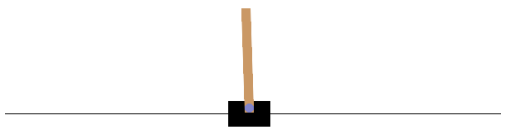
\includegraphics[width=.8\linewidth]{images/cart-pole.png}
    \captionof{figure}{Random observed environment state.}
    \label{fig:cart-pole}
\end{minipage}

\vspace{0.2cm}

The cart-pole environment (seen in Figure \ref{fig:cart-pole}) is a part of the \textit{Gymnasium} package in python. This package contains a number of different virtual environments which can be imported and used to train and validate ones own reinforcement agents. \cite{Gymnasium} \cite{Cart-pole} The environment is created and initialized by the following lines of python code:

\vspace{0.2cm}

\begin{lstlisting}
    import gymnasium as gym

    environment = gym.make('CartPole-v1', render_mode="rgb_array")
    state, _ = environment.reset()
\end{lstlisting}

The agent controls the cart movement, \textit{i.e.}, by pushing it one way or another. The action is therefore binary, being $0$ or $1$ for respectively pushing the cart to the left or the right. By being able to observe the current state of the cart position, cart velocity, pole angle and pole angular velocity, the agent has to choose an appropriate action. A reward is given for every time-step until the pole is no longer standing. The termination (or truncation) is determined by whether the pole angle is greater than $\pm 12 ^\circ$, the cart position is more than $\pm 2.4$ (too far away), or the episode length is greater than $500$ time-steps.

\subsection*{Policy-based gradient agent}
\begin{leftbar}
    Training the policy-based agent by playing $10 000$ games led to a surprisingly good performance. The agent was trained with the \textit{RMSprop} optimizer with a learning-rate of $0.00025$ and a reward discount of $0.99$. See Figure \ref{fig:policy-based-metrics} in the \hyperlink{sec:results}{results}.
\end{leftbar}
\subsection*{Value-based Q-learning agent}
\begin{leftbar}
    \textbf{\textcolor{red}{NOT DONE}}
\end{leftbar}

\newpage
\printbibliography

\newpage
\hypertarget{sec:results}{}
\section*{Results}

\begin{figure}[h]
    \centering
    \begin{minipage}{0.5\textwidth}
        \centering
        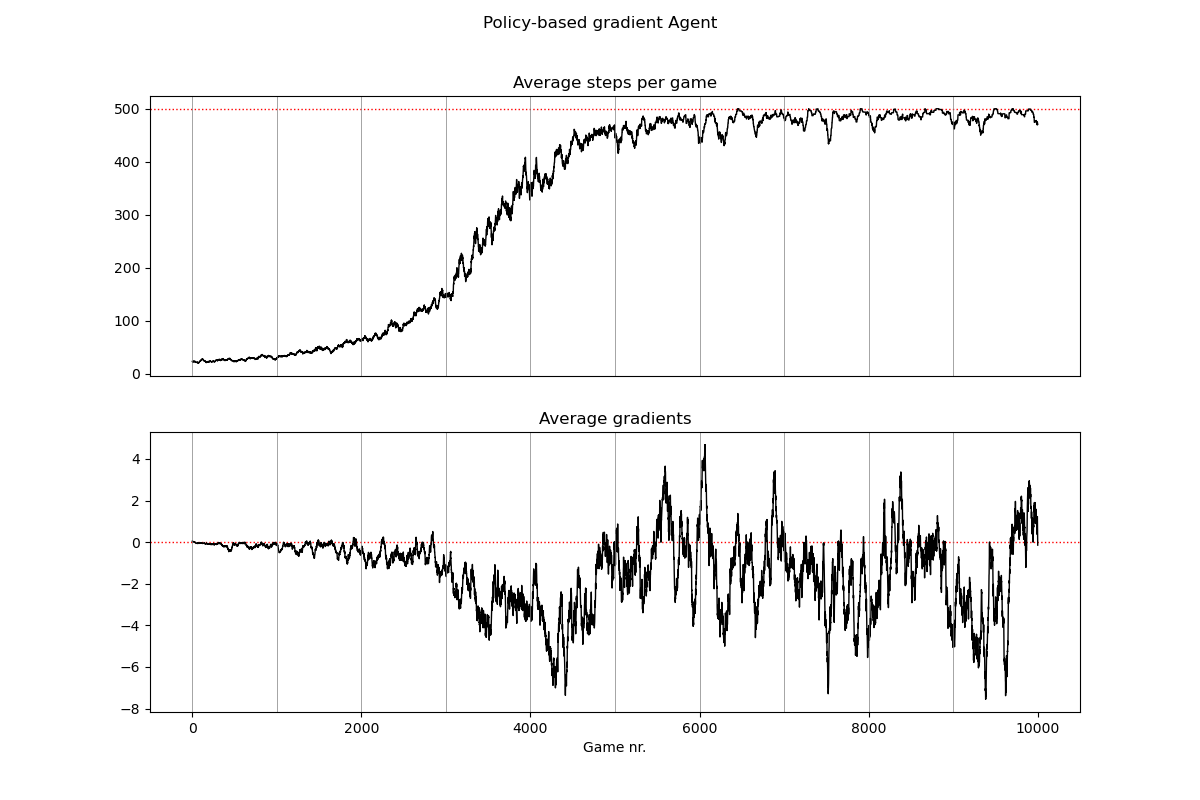
\includegraphics[width=\linewidth]{images/policy-based-gradient.png}
        \caption{Training of the policy-based agent.}
        \label{fig:policy-based-metrics}
    \end{minipage}\hfill
    \begin{minipage}{0.5\textwidth}
        \centering
        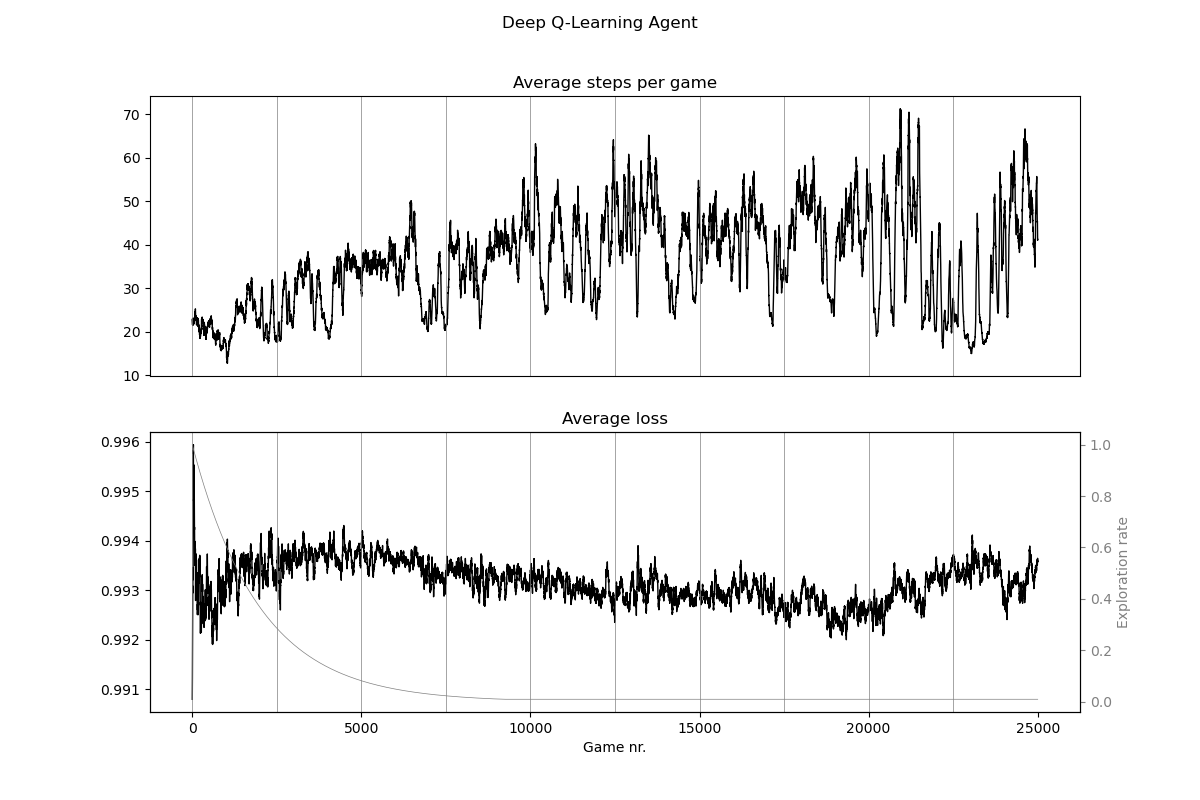
\includegraphics[width=\linewidth]{images/deep-q-agent.png}
        \caption{Training of the value-based agent.}
        \label{fig:value-based-metrics}
    \end{minipage}
\end{figure}

\newpage
\hypertarget{sec:code}{}
\section*{Code}

\end{document}
